% !TEX spellcheck=en_US
\documentclass[a4paper]{article}
\usepackage[american]{babel}
\usepackage[T1]{fontenc}
\usepackage[utf8]{inputenc}
\usepackage[activate={true,nocompatibility},final,tracking=true,kerning=true,spacing=true,factor=1100,stretch=10,shrink=10]{microtype}
\usepackage{fancyhdr}
\usepackage{graphicx}
\usepackage[table]{xcolor}
\usepackage{caption}
\usepackage{subcaption}
\usepackage{csquotes}
\usepackage{hyperref}
\usepackage{textcomp}
\usepackage{verbatim}
\usepackage{xspace}
\usepackage[acronym]{glossaries}

% variables
\newcommand*{\dorg}{Team Havel}
\newcommand*{\dauthor}{Stefan Greve}
\newcommand*{\dtitle}{Git Workshop for Beginners}
\newcommand*{\dversion}{v0.1}

% header
\pagestyle{fancy}
\fancyhf{}
\rhead{\texttt{\dversion}}
\lhead{\dtitle}
\cfoot{Page \thepage}

% colors
\definecolor{lightgray}{rgb}{0.9725,0.9725,0.9725}
\definecolor{nexusred}{HTML}{B80F2E}

% misc macros
\newcommand*{\pref}[2]{#1 (\ref{#2})}
\newcommand*{\flag}[1]{{-}{-}#1}
\newcommand*{\icli}[1]{\textcolor{nexusred}{\texttt{#1}}}
\newcommand*{\cli}[1]{\quad\icli{#1}}
\newcommand*{\home}{\raisebox{0.5ex}{\texttildelow}}
\newcommand*{\carret}{\textbackslash r\xspace}
\newcommand*{\linefeed}{\textbackslash n\xspace}

% microtype
\SetTracking{encoding={*}, shape=sc}{0}

\setacronymstyle{short-long}
\makenoidxglossaries

\include{acronyms}

\begin{document}

\begin{titlepage}
	\centering
	{\scshape\Huge\bfseries{\dorg}\par}
	\par\vspace{3cm}
	
\includegraphics[width=0.45\textwidth]{images/logo.jpg}\par
	\vspace{3cm}
	{\huge\bfseries\dtitle\par}
	\vspace{1cm}
	{\LARGE\itshape\dauthor\par}
	\vspace{1cm}
	{\large\today\par}
	\vfill
	\begin{abstract}
		\texttt{git} is a mature, actively maintained open-source project originally
		developed by Linus Torvald, whose most notably known for creating the Linux
		kernel. The purpose of this document is to help you understand when and how
		to use distributed version control systems in your projects by way of example.
	\end{abstract}
\end{titlepage}

\newpage

\printnoidxglossary[type=\acronymtype]

\newpage

\microtypesetup{protrusion=false}
\tableofcontents
\microtypesetup{protrusion=true}

\newpage

% === Begin Section Includes ===

\section{Preamble}\label{preamble}

\begin{flushleft}
	This workshop does not require any prior exposure to programming, though it would
	certainly be beneficial to you if you have used the command line before. In an ideal
	world everyone would be using a Linux-based operating system, but I am willing to make
	allowances for Windows users this time. With very few exceptions, most of the commands
	you find here work on any modern operating system. While there are many GUI clients for
	Git out there, it is not a stretch to say that nothing beats the terminal experience
	where it is meant to be used.
\end{flushleft}

\begin{flushleft}
	If you have never used the terminal before but you're keen on learning more about it
	then to jump to \pref{section}{powershell} if you're on a Windows machine, else go to
	\pref{section}{bash} (Linux and macOS\footnote{In 2019, Apple changed the default shell
		in macOS Catalina to zsh, although Bash currently remains available as an alternative
		shell.}).
\end{flushleft}


\section{Configuration}\label{configuation}

\begin{flushleft}
	Git uses a series of configuration files to determine non-default behavior. There
	are three different configuration levels, each of which serves a different purpose.
	Note that higher-level configuration settings take precedence over their children.
\end{flushleft}

\begin{enumerate}
	\item \icli{\flag{system}} controls the settings for all users and all repositories on your computer
	\item \icli{\flag{global}} controls the settings for the currently logged-in user and all his repositories
	\item \icli{\flag{local}} controls the settings for the repository it resides in
\end{enumerate}

\begin{flushleft}
	One of the things you want to set first is an username and an email address
	to help Git identify you as the author. Most of the time, it is recommended
	to store these settings in the global configuration file.
\end{flushleft}

\begin{flushleft}
	\cli{git config \flag{global} user.name <username>}
\end{flushleft}
\vspace{-0.6cm}
\begin{flushleft}
	\cli{git config \flag{global} user.email <email>}
\end{flushleft}

\begin{flushleft}
	If you configure a new account on a machine where Git hasn't been used before,
	make sure to set master as the default branch name everywhere.
\end{flushleft}

\begin{flushleft}
	\cli{git config \flag{global} init.defaultBranch master}
\end{flushleft}

\begin{flushleft}
	Other than that there are a few more settings you may want to tweak, though there
	are much more user-specific because they depend on the environment you're operating
	in. The core editor is the editor Git will use when you want to write a multiline
	commit message. For example, if VS Code is your editor of choice you would want to write:
\end{flushleft}

\begin{flushleft}
	\cli{git config \flag{global} core.editor "code \flag{new-window} \flag{wait}"}
\end{flushleft}

\begin{flushleft}
	Another important configuration you want to make helps you avoid line-ending
	issues if you work on cross-platform projects. Even if you're not involved in
	cross-platform projects at the moment, it's better to settle this matter now
	before any problems start to surface later down the line.
\end{flushleft}

\begin{flushleft}
	Windows uses both a carriage-return character (\icli{\carret}) and a linefeed character
	(\icli{\linefeed}) for newlines in its files (CRLF), whereas macOS and Linux systems only
	use the linefeed character (LF). Git can handle this by auto-converting CRLF line endings into LF
	when you add a file to the index, and vice versa when it checks out code onto your filesystem. You
	can turn on this functionality with the \icli{core.autocrlf} setting. If you’re on a Windows machine,
	set it to \icli{true} -- this converts LF endings into CRLF when you check out code:
\end{flushleft}

\begin{flushleft}
	\cli{git config \flag{global} core.autocrlf true}
\end{flushleft}

\begin{flushleft}
	If you're on a Linux or macOS system that uses LF line endings, then you don’t want Git to automatically
	convert them when you check out files; however, if a file with CRLF endings accidentally gets introduced,
	then you may want Git to fix it. You can tell Git to convert CRLF to LF on commit but not the other way
	around by setting \icli{core.autocrlf} to \icli{input}:
\end{flushleft}

\begin{flushleft}
	\cli{git config \flag{global} core.autocrlf input}
\end{flushleft}

\begin{flushleft}
	This setup should leave you with CRLF endings in Windows checkouts, but LF endings on macOS and Linux
	systems and in the repository. If you're a Windows programmer doing a Windows-only project, then you
	can turn off this functionality, recording the carriage returns in the repository by setting \icli{core.autocrlf}
	to \icli{false}:
\end{flushleft}

\begin{flushleft}
	\cli{git config \flag{global} core.autocrlf false}
\end{flushleft}

\subsection{Alias}

\begin{flushleft}
	One of the major advantages of using Git from the terminal is that you can easily
	define your own commands that suits your needs best. See below a list of aliases
	I frequently use in my day-to-day work.
\end{flushleft}

\begin{flushleft}
	Unstage a file without discarding any changes:
\end{flushleft}

\begin{flushleft}
	\cli{git config \flag{global} alias.unstage 'reset HEAD {-}{-}'}
\end{flushleft}

\begin{flushleft}
	Uncommit a file without discarding any changes:
\end{flushleft}

\begin{flushleft}
	\cli{git config \flag{global} alias.uncommit 'reset \flag{soft} HEAD\^{}1'}
\end{flushleft}

\begin{flushleft}
	Show the last commit:
\end{flushleft}

\begin{flushleft}
	\cli{git config \flag{global} alias.last 'log -1 HEAD'}
\end{flushleft}

\begin{flushleft}
	Display log history as graph. Can be extended through the \icli{\flag{branches} \flag{tags}}
	and \icli{\flag{all}} flags, making the output of this command increasingly verbose:
\end{flushleft}

\begin{flushleft}
	\hbox{\cli{git config \flag{global} alias.graph 'log \flag{graph} \flag{oneline} \flag{decorate}'}}
\end{flushleft}

\subsection{Dotfiles Repository}\label{dotfiles-repository}

\begin{flushleft}
	A dotfile repository is a special repository Linux user use to store configuration
	files.
\end{flushleft}

\begin{flushleft}
	Create a new dotfiles repository:
\end{flushleft}

\begin{flushleft}
	\cli{mkdir -p \home/documents/repos}
\end{flushleft}
\vspace{-0.6cm}
\begin{flushleft}
	\cli{git init \flag{bare} \home/documents/dotfiles}
\end{flushleft}

\begin{flushleft}
	Then add this line to \icli{\home/.bashrc}:
\end{flushleft}

\begin{flushleft}
	\hbox{\cli{alias config="/usr/bin/git \flag{git-dir}=\home/documents/repos/dotfiles \flag{work-tree}=\$HOME"}}
\end{flushleft}

\begin{flushleft}
	Next run
\end{flushleft}

\begin{flushleft}
	\cli{config config \flag{local} status.showUntrackedFiles no}
\end{flushleft}

\begin{flushleft}
	Now, to add new configuration files, use the \icli{config} alias:
\end{flushleft}

\begin{flushleft}
	\cli{config add <file>}
\end{flushleft}
\vspace{-0.6cm}
\begin{flushleft}
	\cli{config commit -m <msg>}
\end{flushleft}
\vspace{-0.6cm}
\begin{flushleft}
	\cli{config push}
\end{flushleft}

\begin{flushleft}
	To access your dotfiles from a new machine, run through the following steps:
\end{flushleft}

\begin{flushleft}
	\cli{cd \home/documents/repos}
\end{flushleft}
\vspace{-0.6cm}
\begin{flushleft}
	\cli{git clone \flag{bare} <url> ./dotfiles}
\end{flushleft}

\begin{flushleft}
	Define the \icli{config} alias temporarily in your current shell session:
\end{flushleft}

\begin{flushleft}
	\hbox{\cli{alias config="/usr/bin/git \flag{git-dir}=\home/documents/repos/dotfiles \flag{work-tree}=\$HOME"}}
\end{flushleft}

\begin{flushleft}
	Hide all untracked files on your home director:
\end{flushleft}

\begin{flushleft}
	\cli{cd \home{} \&\& config config \flag{local} status.showUntrackedFiles no}
\end{flushleft}

\begin{flushleft}
	Removes	your local \icli{\home/.bashrc} and \icli{\home/.bash\_profile} files.
	If this is not what you want, rename and/or backup these files. This step is
	mandatory to checkout the branch on the dotfiles repository.
\end{flushleft}

\begin{flushleft}
	\cli{rm .bashrc .bash\_profile}
\end{flushleft}
\vspace{-0.6cm}
\begin{flushleft}
	\cli{config checkout}
\end{flushleft}
\vspace{-0.6cm}
\begin{flushleft}
	\cli{source \home/.bashrc}
\end{flushleft}


\section{SSH Keys}

\begin{flushleft}
	SSH keys are used for for many different things, \textit{inter alia}
\end{flushleft}

\begin{itemize}
	\item \textbf{Remote Access:} SSH ensures encrypted remote connections for users
	      and processes.
	\item \textbf{File Transfer:} SFTP, a secure file transfer protocol managed by SSH,
	      provides a safe way to manipulate files over a network.
	\item \textbf{Port Forwarding:} By mapping a client's port to the server's remote ports,
	      SSH helps secure other network protocols, such as TCP/IP.
	\item \textbf{Tunneling:} This encapsulation technique provides secure data transfers.
	      Tunneling is useful for accessing business-sensitive data online materials from unsecured
	      networks, as it can act as a handy alternative to VPN.
	\item \textbf{Network Management:} The SSH protocol manages network infrastructure and
	      other parts of the system.
\end{itemize}

\begin{flushleft}
	The two most common SSH user authentication methods used are passwords and SSH keys.
	The clients safely send encrypted passwords to the server. However, passwords are a
	risky authentication method because their strength depends on the user’s awareness of
	what constitutes a strong password. Asymmetrically encrypted SSH public-private key
	pairs are a more secure alternative to using passwords. As of August 12th, 2021 GitHub
	made the move to permanently shut down password authentication due to security concerns.
	While you can use a token-based authentication method in its place, using a passphrase
	protected SSH key are by and large still the better alternative if security is means
	anything to you. Many hosting services such as GitHub and GitLab allow you to revoke
	an active SSH key in case of loss or security breach.
\end{flushleft}

\begin{flushleft}
	First create an SSH key with a passphrase for easier authentication\footnote{if you're on Windows,
		use the Git Bash terminal. If you don't have access to WSL, copy and paste the relevant
		sections by hand.}:
\end{flushleft}

\begin{flushleft}
	\cli{ssh-keygen -t rsa -b 4096 -C \$(eval xclip -sel clip -o)}
\end{flushleft}

\begin{flushleft}
	Next start the SSH agent:
\end{flushleft}

\begin{flushleft}
	\cli{eval \$(ssh-agent -s)}
\end{flushleft}

\begin{flushleft}
	Then add and test the SSH key:
\end{flushleft}

\begin{flushleft}
	\cli{ssh-add \home/.ssh/id\_rsa}
\end{flushleft}

\begin{flushleft}
	\cli{ssh -T git@github.com}
\end{flushleft}

\begin{flushleft}
	If you didn't run into any errors in the previous step, go ahead and copy the public key to clipboard:
\end{flushleft}

\begin{flushleft}
	\cli{cat \home/.ssh/id\_rsa.pub | xclip -sel clip}
\end{flushleft}

\begin{flushleft}
	After that open \href{https://github.com/}{GitHub} and navigate to \texttt{Settings}.
	Click on the \texttt{SSH and GPG keys} tab, add your public key and give
	it a descriptive name. Starting the SSH agent for every shell session can be
	annoying sometimes, but you can configure your terminal to automatically start
	the SSH key agent with each new shell session. On Linux, it's as easy as adding
\end{flushleft}

\begin{flushleft}
	\cli{eval \$(eval ssh-agent) > dev/null 2>\&1}
\end{flushleft}

\begin{flushleft}
	your \texttt{\home/.bashrc} file. In addition to that you also need to run
\end{flushleft}

\begin{flushleft}
	\cli{echo "AddKeysToAgent yes" >> \home/.ssh/config}
\end{flushleft}

\begin{flushleft}
	Another advantage of using SSH keys is that they make it much easier to handle
	user authentication for different accounts in a shared environment. This solution
	also works accross many different hosting services, \textit{e.g.} if you want to
	keep your private GitHub account separated from your work account:
	\textcolor{gray}{{\small\verbatiminput{files/config}}}
\end{flushleft}


\section{Semantic Versioning}

\begin{flushleft}
	\emph{The section has been adapted from the website \url{https://semver.org/}
		which formally defines a widely used standard for versioning releases. While there
		exists many other versioning schemes (TeX uses an idiosyncratic version numbering
		system while Microsoft Office build numbers use a date of release format), semantic
		versioning proposes a sequence-based identification scheme with an heavy emphasize on
		significance of compatibility rather than change.}
\end{flushleft}

\begin{flushleft}
	In the world of software management there exists a dreaded place called ``dependency hell.''
	The bigger your system grows and the more packages you integrate into your software, the
	more likely you are to find yourself, one day, in this pit of despair.
\end{flushleft}

\begin{flushleft}
	In systems with many dependencies, releasing new package versions can quickly become a nightmare.
	If the dependency specifications are too tight, you are in danger of version lock (the inability
	to upgrade a package without having to release new versions of every dependent package). If
	dependencies are specified too loosely, you will inevitably be bitten by version promiscuity
	(assuming compatibility with more future versions than is reasonable). Dependency hell is where
	you are when version lock and/or version promiscuity prevent you from easily and safely moving
	your project forward.
\end{flushleft}

\begin{flushleft}
	As a solution to this problem, we propose a simple set of rules and requirements that dictate
	how version numbers are assigned and incremented. These rules are based on but not necessarily
	limited to pre-existing widespread common practices in use in both closed and open-source software.
	For this system to work, you first need to declare a public API. This may consist of documentation
	or be enforced by the code itself. Regardless, it is important that this API be clear and precise.
	Once you identify your public API, you communicate changes to it with specific increments to your
	version number. Consider a version format of X.Y.Z (Major.Minor.Patch). Bug fixes not affecting
	the API increment the patch version, backwards compatible API additions/changes increment the minor
	version, and backwards incompatible API changes increment the major version.
\end{flushleft}

\begin{flushleft}
	We call this system ``Semantic Versioning.'' Under this scheme, version numbers and the way they
	change convey meaning about the underlying code and what has been modified from one version to the
	next.
\end{flushleft}

\begin{flushleft}
	Given a version number \icli{MAJOR.MINOR.PATCH}, increment the:
\end{flushleft}

\begin{enumerate}
	\item \icli{MAJOR} version when you make incompatible API changes,
	\item \icli{MINOR} version when you add functionality in a backwards compatible manner, and
	\item \icli{PATCH} version when you make backwards compatible bug fixes.
\end{enumerate}

\begin{flushleft}
	Additional labels for pre-release and build metadata are available as extensions to the
	\icli{MAJOR.MINOR.PATCH} format.
\end{flushleft}


\section{Core Commands}\label{git-core-commands}

\begin{flushleft}
	\emph{All commands outlined in this section are part of many common Git workflows.
		Simply put, they are worth memorizing because you'll find yourself typing them
		into the console very often before you even know it.}
\end{flushleft}

\begin{flushleft}
	Initialize a new repository:
\end{flushleft}

\begin{flushleft}
	\cli{git init [path]}
\end{flushleft}

\begin{flushleft}
	Clone a repository:
\end{flushleft}

\begin{flushleft}
	\cli{git clone <url> [path]}
\end{flushleft}

\begin{flushleft}
	Stage a file, or all at once:
\end{flushleft}

\begin{flushleft}
	\cli{git add <path|\flag{all}>}
\end{flushleft}

\begin{flushleft}
	Commit all files in the staging area; use the \icli{-m} flag for short commit messages.
\end{flushleft}

\begin{flushleft}
	\cli{git commit [-m <msg>]}
\end{flushleft}

\begin{flushleft}
	Rename a file:
\end{flushleft}

\begin{flushleft}
	\cli{git mv <oldpath> <newnpath>}
\end{flushleft}

\begin{flushleft}
	Remove a file:
\end{flushleft}

\begin{flushleft}
	\cli{git rm <path>}
\end{flushleft}

\begin{flushleft}
	Stage a new file and append it to the last commit. Useful if you forgot to
	change something. Note that you have to force push this commit if it was
	already pushed previously. As a rule of thumb, you should never force push
	anything unless you're aware of all the negative side effects this option
	can cause.
\end{flushleft}

\begin{flushleft}
	\cli{git add <file>}
\end{flushleft}
\vspace{-0.4cm}
\begin{flushleft}
	\cli{git commit \flag{amend} \flag{no-edit}}
\end{flushleft}

\begin{flushleft}
	Edit the last commit message. Because this action also irreversibly changes
	Git's history in retrospective, the aforementioned warning also applies here.
\end{flushleft}

\begin{flushleft}
	\cli{git commit \flag{amend}}
\end{flushleft}

\begin{flushleft}
	Push your commits to a remote repository:
\end{flushleft}

\begin{flushleft}
	\cli{git push [\flag{force}]}
\end{flushleft}

\begin{flushleft}
	Create a new branch based off the current branch:
\end{flushleft}

\begin{flushleft}
	\cli{git checkout -b <branch>}
\end{flushleft}

\begin{flushleft}
	Push the current branch and set the remote as upstream. An upstream is an another
	branch name, usually a remote-tracking branch, associated with a local branch.
\end{flushleft}

\begin{flushleft}
	\cli{git push \flag{set-upstream} origin <branch>}
\end{flushleft}


\section{Miscellaneous Commands}\label{git-misc-commands}

% === git remote

\subsection{Remotes}\label{git-remote}

\begin{flushleft}
	Change the remote URL on a local repository (here: \icli{origin}):
\end{flushleft}

\begin{flushleft}
	\cli{git remote set-url origin <url>}
\end{flushleft}

\begin{flushleft}
	Remove a remote:
\end{flushleft}

\begin{flushleft}
	\cli{git remote rm <remote>}
\end{flushleft}

% === git branch

\subsection{Branches}\label{git-branch}

\begin{flushleft}
	Rename the active branch:
\end{flushleft}

\begin{flushleft}
	\cli{git branch -m <newname>}
\end{flushleft}

\begin{flushleft}
	If you want to rename this branch on GitHub as well, run additionally:
\end{flushleft}

\begin{flushleft}
	\cli{git push origin -u <newname>}
\end{flushleft}

\begin{flushleft}
	To check out a branch from GitHub, use:
\end{flushleft}

\begin{flushleft}
	\cli{git fetch \flag{all}}
\end{flushleft}
\vspace{-0.4cm}
\begin{flushleft}
	\cli{git checkout -b <branch> origin/<branch>}
\end{flushleft}

\begin{flushleft}
	Delete a local and remote branch:
\end{flushleft}

\begin{flushleft}
	\cli{git branch \flag{delete} <branch>}
\end{flushleft}
\vspace{-0.4cm}
\begin{flushleft}
	\cli{git push origin \flag{delete} <branch>}
\end{flushleft}

% === git tag

\subsection{Tags}\label{git-tag}

\begin{flushleft}
	Add a new tag:
\end{flushleft}

\begin{flushleft}
	\cli{git tag <version>}
\end{flushleft}

\begin{flushleft}
	Add a new annotated tag:
\end{flushleft}

\begin{flushleft}
	\cli{git tag -a <version> -m <msg>}
\end{flushleft}

\begin{flushleft}
	Add a new annotated tag to a previous commit:
\end{flushleft}

\begin{flushleft}
	\cli{git tag -a <version> -m <msg> <sha>}
\end{flushleft}

\begin{flushleft}
	Push a specific tag to remote:
\end{flushleft}

\begin{flushleft}
	\cli{git push origin <version>}
\end{flushleft}

\begin{flushleft}
	Push all tags to remote:
\end{flushleft}

\begin{flushleft}
	\cli{git push origin \flag{tags}}
\end{flushleft}

\begin{flushleft}
	Delete a local tag:
\end{flushleft}

\begin{flushleft}
	\cli{git tag \flag{delete} <version>}
\end{flushleft}

\begin{flushleft}
	Delete a remote tag:
\end{flushleft}

\begin{flushleft}
	\cli{git push \flag{delete} origin <version>}
\end{flushleft}

% === git log

\subsection{Logs}\label{git-log}

\begin{flushleft}
	Display all commits from a particular author:
\end{flushleft}

\begin{flushleft}
	\cli{git log \flag{author}=<name> \flag{oneline}}
\end{flushleft}

\begin{flushleft}
	Get commits in a time range using Ruby expressions:
\end{flushleft}

\begin{flushleft}
	\cli{git log \flag{after} 10.days.ago \flag{oneline}}
\end{flushleft}

\begin{flushleft}
	View commit history as ASCII graph:
\end{flushleft}

\begin{flushleft}
	\cli{git log \flag{graph}}
\end{flushleft}

\begin{flushleft}
	Format log output:
\end{flushleft}

\begin{flushleft}
	\cli{git log \flag{pretty}:"<options>"}
\end{flushleft}

\begin{flushleft}
	See also this \url{https://git-scm.com/docs/pretty-formats} for more information.
\end{flushleft}

% === git diff

\subsection{Diffs}\label{git-diffs}

\begin{flushleft}
	Inspect diff statistics:
\end{flushleft}

\begin{flushleft}
	\cli{git diff \flag{stat}}
\end{flushleft}

\begin{flushleft}
	View the diff stats from last month:
\end{flushleft}

\begin{flushleft}
	\cli{git diff \flag{numstat} "\@{1 month ago}"}
\end{flushleft}

\begin{flushleft}
	View diffs from staged files; note that without this last flag nothing would be displayed:
\end{flushleft}

\begin{flushleft}
	\cli{git diff \flag{staged}}
\end{flushleft}

\begin{flushleft}
	View diffs between two branches:
\end{flushleft}

\begin{flushleft}
	\cli{git diff [\flag{name-only}] master...<branch>}
\end{flushleft}

\begin{enumerate}
	\item the \icli{\flag{name-only}} options only lists modified files without its diffs
	\item this syntax also works for comparing tags (with branches or other tags)
	\item the order of branches matters: \icli{<target-branch>...<active-branch>}
	\item the command \icli{git diff ..master} compares the checked-out branch to \icli{master}
\end{enumerate}

\begin{flushleft}
	You can refine this diffs even more with
\end{flushleft}

\begin{flushleft}
	\cli{git diff ..master {-}{-} <path> }
\end{flushleft}

% === git submodule

\subsection{Submodules}\label{git-submodule}

\begin{flushleft}
	Add a new submodule:
\end{flushleft}

\begin{flushleft}
	\cli{git submodule add <url>}
\end{flushleft}

\begin{flushleft}
	Update all submodules (after a pull):
\end{flushleft}

\begin{flushleft}
	\cli{git submodule update \flag{init} \flag{recursive}}
\end{flushleft}

\begin{flushleft}
	Submodules are removed the same way you would remove any file in Git.
\end{flushleft}

% === git stash

\subsection{Stash}\label{git-stash}

\begin{flushleft}
	This command is very useful if you want to change branches without having to
	commit or discard any changes made locally. See also the example at the end of
	this subsection for a more basic rundown and hands-on example on how to use this
	command.
\end{flushleft}

\begin{flushleft}
	\cli{git stash [\flag{include-untracked}|\flag{all}|\flag{path} <file(s)>]}
\end{flushleft}

\begin{flushleft}
	By default, this command ignores untracked or ignored files. If you don't want
	that, make sure to add the \icli{\flag{include-untracked}} option to also include
	untracked files as well (or use the  \icli{\flag{all}} option if you want to stash
	all untracked \emph{and} ignored files). To stash specific files, use the \icli{\flag{patch}}
	option which accepts one or more file paths.
\end{flushleft}

\begin{flushleft}
	You can review your stash with the
\end{flushleft}

\begin{flushleft}
	\cli{git stash list}
\end{flushleft}

\begin{flushleft}
	command which are stored using a LIFO strategy. By default, stashes are marked as
	WIP on top of the branch and commit that you created the stash from. However, this
	limited amount of information isn't helpful when you have multiple stashes, as it
	becomes difficult to remember or individually check their contents. To add a description
	to the stash, you can use the command
\end{flushleft}

\begin{flushleft}
	\cli{git stash save <description>}
\end{flushleft}

\begin{flushleft}
	As the name implies, this command applies the topmost stash (if no ID is specified):
\end{flushleft}

\begin{flushleft}
	\cli{git stash apply}
\end{flushleft}

\begin{flushleft}
	You can target a specific stash using stash IDs. The above command, for instance,
	is equivalent to
\end{flushleft}

\begin{flushleft}
	\cli{git stash apply@\{0\}}
\end{flushleft}

\begin{flushleft}
	The \icli{pop} command is similar \icli{apply}, but does one more thing in sequence:
	after applying the patch it drops this stash from the list. However, if there are
	conflicts when a stash is popped, \icli{pop} will not remove the stash.
\end{flushleft}

\begin{flushleft}
	\cli{git stash pop}
\end{flushleft}

\begin{flushleft}
	If you have multiple stashes, you can inspect the diff with the \icli{show} command.
	The \icli{\flag{path}} flag is optional here and produces a more verbose output.
\end{flushleft}

\begin{flushleft}
	\cli{git stash show stash@\{0\} [\flag{patch}]}
\end{flushleft}

\begin{flushleft}
	You can pass a stash ID to delete an individual stash from the stash list. For
	example, to remove the second stash run:
\end{flushleft}

\begin{flushleft}
	\cli{git stash drop@\{1\}}
\end{flushleft}

\begin{flushleft}
	To clear the entire stash, use:
\end{flushleft}

\begin{flushleft}
	\cli{git stash clear}
\end{flushleft}

\subsubsection{Switching Branches on the Fly}

\begin{flushleft}
	In this scenario, you are currently on the \icli{feature-01} branch, but want
	to check out the \icli{feature-02} branch with a untracked changes in your
	current directory:
\end{flushleft}

\begin{flushleft}
	\cli{git stash \flag{all}}
\end{flushleft}
\vspace{-0.6cm}
\begin{flushleft}
	\cli{git checkout feature-02}
\end{flushleft}
\vspace{-0.6cm}
\begin{flushleft}
	\cli{\# taking a quick gander here :)}
\end{flushleft}
\vspace{-0.6cm}
\begin{flushleft}
	\cli{git checkout feature-01}
\end{flushleft}
\vspace{-0.6cm}
\begin{flushleft}
	\cli{git stash pop}
\end{flushleft}

% === git clean

\subsection{Clean}\label{git-clean}

\begin{flushleft}
	Remove all untracked files. If the Git variable \icli{clean.requireForce} is
	not set to \icli{false}, \icli{clean} will refuse to delete files or directories
	unless a second \icli{-f} is given.
\end{flushleft}

\begin{flushleft}
	\cli{git clean <-i|-n|-f> -d .}
\end{flushleft}

\begin{itemize}
	\item \icli{-i} (or \icli{\flag{interactive}}) will show what would be done and clean files interactively
	\item \icli{-n} (or \icli{\flag{dry-run}}) will not remove anything and only show what would be done
	\item \icli{-f} (or \icli{\flag{force}}) will set \icli{clean.requireForce} to false
\end{itemize}


\section{Bash}\label{bash}

\begin{flushleft}
	\emph{Bash is the GNU Project's shell and short for the Bourne Again SHell.
		As of today, Bash is the most popular shell among Linux users. Due to its
		popularity and widespread usage, Bash has also been ported to Windows and
		distributed with \href{https://cygwin.com/}{Cygwin} and
		\href{https://osdn.net/projects/mingw/}{MinGW}. As opposed to Windows,
		UNIX is an entire ecosystem self-tuned around text files.}
\end{flushleft}

\subsection{Profile Setup}\label{bash-profile}

\begin{flushleft}
	On most systems, \icli{\home/.bashrc} is only used when you startup an interactive
	non-login shell. However, if you open a new shell it is often an interactive login
	shell which completely ignores your configuration in \icli{\home/.bashrc} unless
	source the \icli{\home/.bashrc} from your \icli{\home/.profile} or \icli{\home/.bash\_profile}
	file:
\end{flushleft}

\begin{flushleft}
	\cli{[[ -f \home/.bashrc ]] \&\& .\, \home/.bashrc}
\end{flushleft}

\subsection{Core Commands}\label{bash-core-commands}

\begin{flushleft}
	Create a new file:
\end{flushleft}

\begin{flushleft}
	\cli{touch <file>}
\end{flushleft}

\begin{flushleft}
	Initialize a \icli{txt} file with a string value:
\end{flushleft}

\begin{flushleft}
	\cli{echo "Hello, World!" > test.txt}
\end{flushleft}

\begin{flushleft}
	Print out the content of \icli{test.txt} to standard output:
\end{flushleft}

\begin{flushleft}
	\cli{cat [\flag{number}] test.txt}
\end{flushleft}

\begin{flushleft}
	Print the first ten lines of the file. Pipe the output to \icli{tail} to
	reverse this effect:
\end{flushleft}

\begin{flushleft}
	\cli{cat test.txt | head}
\end{flushleft}

\begin{flushleft}
	Create a new directory. Use the \icli{-p} if one or more parents don't exist.
\end{flushleft}

\begin{flushleft}
	\cli{mkdir [-p] <path>}
\end{flushleft}

\begin{flushleft}
	Move a file to a new location. This Cmdlet can also be used to rename a file:
\end{flushleft}

\begin{flushleft}
	\cli{mv <path> <destination>}
\end{flushleft}

\begin{flushleft}
	List all files in a specific directory. Use the \icli{g} flag for a long listing
	format (excluding the owner), and \icli{\flag{color}=auto} for colorful output.
\end{flushleft}

\begin{flushleft}
	\cli{ls <dir> [-g|\flag{color=auto}]}
\end{flushleft}

\begin{flushleft}
	List all \icli{tex} files from the \icli{src} directory of this document,
	and format the output accordingly.
\end{flushleft}

\begin{flushleft}
	\cli{ls -g {-}{-}  src/**/*.tex}
\end{flushleft}

\begin{flushleft}
	Remove a file:
\end{flushleft}

\begin{flushleft}
	\cli{rm <file>}
\end{flushleft}

\begin{flushleft}
	Remove an empty directory:
\end{flushleft}

\begin{flushleft}
	\cli{rmdir <dir>}
\end{flushleft}

\begin{flushleft}
	Remove a non-empty directory recursively and run this command in a dry-run mode:
\end{flushleft}

\begin{flushleft}
	\cli{rm -rf <dir> \flag{dry-run}}
\end{flushleft}


\section{PowerShell}\label{powershell}

\begin{flushleft}
	\emph{In PowerShell, administrative tasks are generally performed by Cmdlets
		(pronounced command-lets), which are specialized .NET classes implementing a
		particular operation. While bash scripts primarily consume strings and text files,
		PowerShell is centered around the idea of processing and communicating through
		Objects and APIs. It easily integrates into Window's COM interfaces and the .NET
		Framework and is often regarded as the better choice for automating tasks on
		Windows operating system.}
\end{flushleft}

\subsection{Profile Setup}\label{powershell-profile-setup}

\begin{flushleft}
	There are up to six different locations for you to choose when you want to create
	a new PowerShell profile.
\end{flushleft}

\begin{flushleft}
	\cli{\$PROFIE | Get-Member -Type NoteProperty | Format-List *}
\end{flushleft}

\begin{flushleft}
	But first you will want to check if you already have a profile:
\end{flushleft}

\begin{flushleft}
	\cli{Test-Path \$HOME\textbackslash Documents\textbackslash WindowsPowerShell\textbackslash profile.ps1}
\end{flushleft}

\begin{flushleft}
	If the result of this operation is \icli{False}, go ahead and create a new profile:
\end{flushleft}

\begin{flushleft}
	\cli{New-Item -Force \$HOME\textbackslash Documents\textbackslash WindowsPowerShell\textbackslash profile.ps1}
\end{flushleft}

\begin{flushleft}
	Next set the execution policy appropriately so that you can execute your own
	PowerShell scripts:
\end{flushleft}

\begin{flushleft}
	\cli{Set-EexeutionPolicy RemoteSigned}
\end{flushleft}

\begin{flushleft}
	Now open your profile and define a \icli{\$psrc} variable so that you access
	this file more conveniently:
\end{flushleft}

\begin{flushleft}
	\cli{\$gloabl:psrc="\$HOME\textbackslash Documents\textbackslash WindowsPowerShell\textbackslash profile.ps1"}
\end{flushleft}

\subsection{Core Commands}\label{powershell-core-commands}

\begin{flushleft}
	Many PowerShell commands provide a Linux-like alias for common commands:
\end{flushleft}

\begin{flushleft}
	\cli{Get-Alias -Definition <cmdlet>}
\end{flushleft}

\begin{flushleft}
	For example, the \icli{Set-Location} Cmdlet is also accessible using any of
	these abbreviations:
	\textcolor{gray}{{\small\verbatiminput{files/cdalias.txt}}}
\end{flushleft}

\begin{flushleft}
	Create a new file. You can add the \icli{[-ItemType <file|directory>]} option to
	specify the type of file you want to create. Additionally, you can also pass
	the \icli{-Value <string>} option to initialize the file with a string value.
\end{flushleft}

\begin{flushleft}
	\cli{New-Item [-Path <path>] -Name <file>}
\end{flushleft}

\begin{flushleft}
	Move a file to a new location. This Cmdlet can also be used to rename a file:
\end{flushleft}

\begin{flushleft}
	\cli{Move-Item -Path <file> -Destination <file>}
\end{flushleft}

\begin{flushleft}
	Print the content of \icli{test.txt} to standard output:
\end{flushleft}

\begin{flushleft}
	\cli{Get-Content test.txt}
\end{flushleft}

\begin{flushleft}
	List all \icli{tex} files from the \icli{src} directory of this document,
	and format the output accordingly. Note that \icli{gci} and \icli{ft} are
	aliases for \icli{Get-ChildItem} and \icli{Format-Table}, respectively.
\end{flushleft}

\begin{flushleft}
	\cli{gci .\textbackslash src -Include *.tex -Recurse | ft Name, DirectoryName}
\end{flushleft}

\begin{flushleft}
	Remove all log files in the current working directory:
\end{flushleft}

\begin{flushleft}
	\cli{Remove-Item -Path . -Include *.log}
\end{flushleft}

\begin{flushleft}
	Remove all \icli{txt} files in a sub directory:
\end{flushleft}

\begin{flushleft}
	\cli{Get-ChildItem -Path .\textbackslash exmdir\textbackslash{} *.txt -Recurse | Remove-Item}
\end{flushleft}

\begin{flushleft}
	Remove a directory recursively. Use the \icli{-WhatIf} option to enable the
	dry-run	mode:
\end{flushleft}

\begin{flushleft}
	\cli{Remove-Item -Recurse -Force <dir> [-WhatIf]}
\end{flushleft}


\section{Software Licenses}\label{licenses}

\begin{flushleft}
	Every business uses software to manage business processes, communicate with
	employees, customers, and vendors, and for myriad other purposes. In most instances,
	software products require activating licenses or agreeing to ``terms and conditions''
	before programs can be downloaded, installed, or accessed. There are many types
	of software licenses, with different terms, support agreements, restrictions, and
	costs. Users need to understand the basics of software licenses, to ensure a
	full understanding of responsibilities and compliance with legal terms and
	limitations.
\end{flushleft}

\begin{flushleft}
	A software license is a contract between the entity that created and supplied
	an application, underlying source code, or related product and its end user.
	The license is a text document designed to protect the intellectual property
	of the software developer and to limit any claims against them that may arise
	from its use. A software license also provides legally binding definitions for
	the distribution and use of the software. End-user rights, such as installation,
	warranties, and liabilities, are also often spelled out in the software license,
	including protection of the developer's intellectual property.
\end{flushleft}

\subsection{Types of Licenses}\label{license-types}

\begin{flushleft}
	\textbf{Public Domain:} This is the most permissive type of software license.
	When software is in the public domain, anyone can modify and use the software
	without any restrictions. But you should always make sure it's secure before
	adding it to your own codebase. Warning: Code that doesn't have an explicit
	license is NOT automatically in the public domain. This includes code snippets
	you find on the internet.
\end{flushleft}

\begin{flushleft}
	\textbf{Permissive:} Permissive licenses are also known as ``Apache style'' or
	``BSD style.'' They contain minimal requirements about how the software can be
	modified or redistributed. This type of software license is perhaps the most
	popular license used with free and open source software. Aside from the Apache
	License and the BSD License, another common variant is the MIT License.
\end{flushleft}

\begin{flushleft}
	\textbf{LGPL:} The GNU Lesser General Public License allows you to link to open
	source libraries in your software. If you simply compile or link an LGPL-licensed
	library with your own code, you can release your application under any license
	you want, even a proprietary license. But if you modify the library or copy
	parts of it into your code, you'll have to release your application under similar
	terms as the LGPL.
\end{flushleft}

\begin{flushleft}
	\textbf{Copyleft:} Copyleft licenses are also known as reciprocal licenses or
	restrictive licenses. The most well-known example of a copyleft or reciprocal
	license is the GPL. These licenses allow you to modify the licensed code and
	distribute new works based on it, as long as you distribute any new works or
	adaptations under the same software license. For example, a component's license
	might say the work is free to use and distribute for personal use only. So any
	derivative you create would also be limited to personal use only. (A derivative
	is any new software you develop that contains the component.) The catch here is
	that the users of your software would also have the right to modify the code.
	Therefore, you'd have to make your own source code available. But of course,
	exposing your source code may not be in your best interests.
\end{flushleft}

\begin{flushleft}
	\textbf{Propriety:} Of all types of software licenses, this is the most restrictive.
	The idea behind it is that all rights are reserved. It's generally used for
	proprietary software where the work may not be modified or redistributed.
\end{flushleft}

\subsection{Legal Terms}\label{license-legal-terms}

\begin{itemize}
	\item \textbf{Commercial Use:} Describes the ability to use the software for commercial purposes.
	\item \textbf{Modify:} Describes the ability to modify the software and create derivatives.
	\item \textbf{Distribute:} Describes the ability to distribute original or modified (derivative) works.
	\item \textbf{Place Warranty:} Describes the ability to place warranty on the software licensed.
	\item \textbf{Sublicense:} The LGPL prohibits sublicensing, yet each user that receives the software automatically has the right to run, modify and distribute the work.
	\item \textbf{Use Trademark:} You may not use the names of the original company or its members to endorse derived products.
	\item \textbf{Hold Liable:} Describes the warranty and if the software/license owner can be charged for damages.
	\item \textbf{State Changes:} Stating significant changes made to software.
	\item \textbf{Disclose Source:} If you distribute this library in an executable, you must make the source available for 3 years.
	\item \textbf{Include Original:} Describes whether copies of the original software or instructions to obtain copies must be distributed with the software.
	\item \textbf{Include Copyright:} Describes whether the original copyright must be retained.
	\item \textbf{Include License:} Including the full text of license in source or object code copies.
	\item \textbf{Include Install Instructions:} If the software is part of a consumer device, you must include the installation information necessary to modify and reinstall the software.
	\item \textbf{Include Note:} If the library has a "NOTICE" file with attribution notes, you must include that NOTICE when you distribute. You may append to this NOTICE file.
\end{itemize}

\subsection{Copyleft vs Copyright}\label{copyleft-vs-copyright}

\begin{flushleft}
	A copyright is a legal right bestowed upon creators of original works to dictate
	how those works can or cannot be copied, modified, and distributed by others. If
	someone uses or distributes an original work in a way that's contrary to what its
	creator allows (``infringement''), the creator is entitled to seek legal action.
\end{flushleft}

\begin{flushleft}
	Copyleft is a term coined by Richard Stallman who originally used this term to
	distinguish his way of free software licensing (such as GPLv3 or LGPLv3) from
	the other Copyright licenses which are typically designed by proprietary companies
	to keep the holding rights of a software to themselves by not disclosing the source
	code. The Free Software Foundation (FSF) is a  is a nonprofit organization that set
	out to promote the usage and development of free software\footnote{\href{https://www.gnu.org/philosophy/free-sw.html.en}{What is Free Software?}}.
\end{flushleft}

\begin{flushleft}
	It's important to point out that the term copyleft holds no legal significance
	in any court of the world because it was never really defined under the law.
	However, the terms and conditions of copyleft licenses such as GPLv3 are legally
	binding. On a related note, the terms Share-Alike and Copyleft are for the most
	part synonymous, with the exception that Share-Alike licenses are fit for use for
	works of art, while copyleft licenses were designed with software development in
	mind. The main idea behind copyright is that creators restrict what others can or
	cannot do with their works and must grant individual permission to do otherwise.
	Copyleft licenses exist within the legal structure of copyrights and grants the
	user permission to copy, modify and distribute works in any fashion they like.
	Failing to abide to the rules that are governed by copyleft licenses provides
	the project maintainer with legal grounds for action. While copyleft licenses are
	very permissive with regards to the users freedom, it also imposes a series of
	demands that are to be kept up by the developers, which most notably includes
	the requirement that any derivative works must be published under a license that
	grants the same rights as the license of the pulled-in dependency.
\end{flushleft}

\subsection{Common Licenses}\label{common-licenses}

\subsubsection{MIT}

\begin{flushleft}
	If you use the MIT license, you \emph{can} do any of the following:
\end{flushleft}

\begin{enumerate}
	\item Commercial Use
	\item Modify
	\item Sublicense
	\item Private Use
\end{enumerate}

\begin{flushleft}
	If you use the MIT license, you \emph{canont} do any of the following:
\end{flushleft}

\begin{enumerate}
	\item Hold Liable
\end{enumerate}

\begin{flushleft}
	If you use the MIT license, you \emph{must} do all of the following:
\end{flushleft}

\begin{enumerate}
	\item Include Copyright
	\item Include License
\end{enumerate}

% ===

\subsubsection{GPLv3}

\begin{flushleft}
	If you use the GPLv3 license, you \emph{can} do any of the following:
\end{flushleft}

\begin{enumerate}
	\item Commercial Use
	\item Modify
	\item Distribute
	\item Place Warranty
	\item Use Patent Claims
\end{enumerate}

\begin{flushleft}
	If you use the GPLv3 license, you \emph{canont} do any of the following:
\end{flushleft}

\begin{enumerate}
	\item Sublicense
	\item Hold Liable
\end{enumerate}

\begin{flushleft}
	If you use the GPLv3 license, you \emph{must} do all of the following:
\end{flushleft}

\begin{enumerate}
	\item Include Original
	\item State Changes
	\item Disclose Source
	\item Include Copyright
	\item Include License
	\item Include Install Instructions
\end{enumerate}

% ===

\subsubsection{LGPLv3}

\begin{flushleft}
	If you use the LGPLv3 license, you \emph{can} do any of the following:
\end{flushleft}

\begin{enumerate}
	\item Commercial Use
	\item Modify
	\item Distribute
	\item Place Warranty
	\item Use Patent Claims
\end{enumerate}

\begin{flushleft}
	If you use the LGPLv3 license, you \emph{canont} do any of the following:
\end{flushleft}

\begin{enumerate}
	\item Sublicense
	\item Hold Liable
\end{enumerate}

\begin{flushleft}
	If you use the LGPLv3 license, you \emph{must} do all of the following:
\end{flushleft}

\begin{enumerate}
	\item Include Original
	\item State Changes
	\item Disclose Source
	\item Include Copyright
	\item Include License
	\item Include Install Instructions
\end{enumerate}

% ===

\subsubsection{Apache License 2.0}

\begin{flushleft}
	If you use the Apache License 2.0, you \emph{can} do any of the following:
\end{flushleft}

\begin{enumerate}
	\item Commercial Use
	\item Modify
	\item Distribute
	\item Sublicense
	\item Private Use
	\item Place Warranty
\end{enumerate}

\begin{flushleft}
	If you use the Apache License 2.0, you \emph{canont} do any of the following:
\end{flushleft}

\begin{enumerate}
	\item Hold Liable
	\item Use Trademark
\end{enumerate}

\begin{flushleft}
	If you use the Apache License 2.0, you \emph{must} do all of the following:
\end{flushleft}

\begin{enumerate}
	\item Include Copyright
	\item Include License
	\item State Changes
	\item Include Notice
\end{enumerate}

% ===

\subsubsection{BSD-3 Clause (Revised)}

\begin{flushleft}
	If you use the BSD-3 Clause (Revised) license, you \emph{can} do any of the following:
\end{flushleft}

\begin{enumerate}
	\item Commercial Use
	\item Modify
	\item Distribute
	\item Place Warranty
\end{enumerate}

\begin{flushleft}
	If you use the BSD-3 Clause (Revised) license, you \emph{canont} do any of the following:
\end{flushleft}

\begin{enumerate}
	\item Use Trademark
	\item Hold Liable
\end{enumerate}

\begin{flushleft}
	If you use the BSD-3 Clause (Revised), you \emph{must} do all of the following:
\end{flushleft}

\begin{enumerate}
	\item Include Copyright
	\item Include License
\end{enumerate}

\subsection{License Compatibility}

\begin{flushleft}
	Before you can determine which licenses govern any reused code in your codebase,
	you need to create a software bill of materials, or a list of all the components
	in your code. And the fastest way to generate that list is with a software composition
	analysis tool. A good SCA tool will be able to find full components as well as
	code snippets, and it'll tell you which licenses apply to each piece of code and
	whether you might be using licenses that have conflicts.
\end{flushleft}

\begin{flushleft}
	The licences for distributing free or open source software (FOSS) are divided
	in two families: permissive and reciprocal (or ``copyleft''). Permissive licenses
	(BSD, MIT, X11, Apache, Zope) are generally compatible and interoperable with most
	other licences, tolerating to merge, combine or improve the covered code and to
	re-distribute it under many licences (including non-free or ``proprietary'').
\end{flushleft}

\begin{flushleft}
	At the contrary, the reciprocal licences impose to provide back the source code
	under the same license in case of distribution, when the distributed work is
	a derivative of the covered work. To avoid software appropriation by third
	parties, many open source projects have adopted reciprocal licensing terms:
	this is the case of the two Gnu GPLs and the EUPL.
\end{flushleft}

\begin{flushleft}
	Some licences like the LGPL or the MPL try to compromise between the permissive
	and reciprocal requirements: covered components (and their specific derivatives)
	will always keep their primary license, but the combined application ``as a whole''
	(even if it may be considered globally as a derivative) or its executable binary
	(a single program from the user point of view) can be distributed under any license.
\end{flushleft}

\begin{flushleft}
	In most cases, permissive licenses are also compatible with copyleft licenses.
	There are two exceptions to this rule: The Apache 2.0 license and the original
	(4-clause) BSD license. The Apache 2.0's license partner rights make it incompatible
	with GPLv2, but it is compatible with GPLv3. The 4-clause BSD license's advertising
	clause makes it incompatible with all copyleft licenses. The modified (3-clause)
	BSD license doesn't include the problematic advertising clause, so it is compatible.
\end{flushleft}

\begin{flushleft}
	The most problematic practice is combining two copyleft licenses. As a rule of
	thumb, copyleft licenses are incompatible unless they have explicit compatibility
	provisions. As Richard Stallman, creator of the GNU GPL license:
\end{flushleft}

\begin{displaycquote}
	``If license A says extended programs must be under license A, and license B
	says extended programs must be under license B, they have an irreconcilable
	disagreement; the license of the combined program would have to be A, and it
	would have to be B.''
\end{displaycquote}

\begin{flushleft}
	\textbf{Compatibility} is the possibility to combine or merge software code
	covered by several licences and to distribute the combined work. At the contrary,
	license incompatibility exists when a program is derivative of components licensed
	under two different reciprocal licences (for example, the GPLv2, which is still
	the most used copyleft licence, is not compatible with GPLv3, and vice-versa).
\end{flushleft}

\begin{flushleft}
	\textbf{Interoperability} is another legal concept originally defined by Directive
	91/250/EEC as "the ability to exchange information and mutually to use the
	information which has been exchanged" (Recital 10). And to implement interoperability,
	the reproduction of ``interfaces'' (also defined in as ``the parts of the program
	which provide for interconnection and interaction between elements of software'') is
	authorized as a copyright exception to the author's exclusive rights (possibly
	formalized in a copyright license), This is the reason why the EUPL, by application
	of EU law, is interoperable. This is a major difference with some other reciprocal
	licences (mainly the GPLv2, GPLv3 and AGPL) where the license steward states that
	static or dynamic linking extend their copyright.
\end{flushleft}

\begin{flushleft}
	A logical incompatibility issue may be resolved through \textbf{Dual Licensing}: the
	original licensor (owning full copyright) may provide the same program under two or
	more licences, even if these licenses are not compatible. The most frequent cases
	apply to licensors distributing their work under the ``GPL'' (without mentioning
	the version number, or adding "or later"): in such case, recipients can use the
	work under any of these licences (GPLv2 or GPLv3), which is in practice a dual
	licensing. When the licences are mutually incompatible, the risk of dual licensing
	is the forking of the program in various legally incompatible releases, which even
	the original licensor will not be able to reunify.
\end{flushleft}

\begin{figure}[ht]
	\centering
	% https://i.imgur.com/ejucFRV.png
	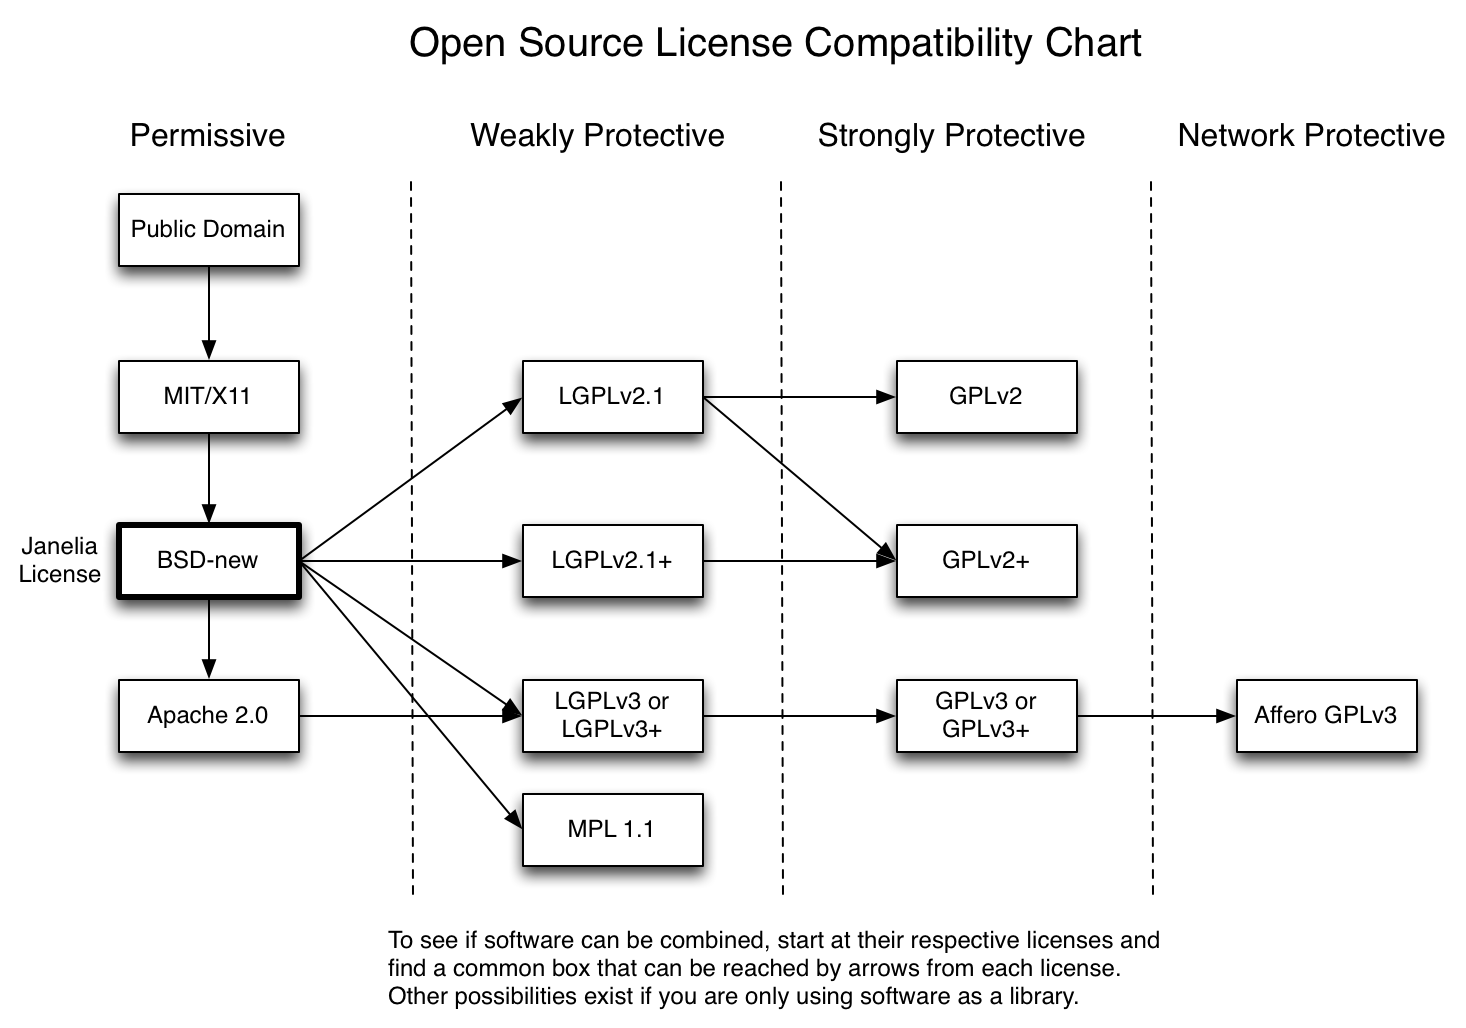
\includegraphics[scale=0.4]{images/open_licenses.png}
	\caption{FOSS License Compatibility}\label{fig:foss-licenses}
\end{figure}

\begin{flushleft}
	In this figure, the boxes are the names of different FLOSS licenses. An arrow
	from box A to box B means that you can combine software with these licenses;
	the combined result effectively has the license of B, possibly with additions
	from A. To see if software can be combined, start at their respective
	licenses, and find a common box by following the arrows. For example, Apache 2.0-licensed
	software and GPLv2+-licensed software can both reach "GPLv3 or GPLv3+", so they
	can be combined using GPLv3 or GPLv3+.
\end{flushleft}


\section{Project Management}\label{project-management}

\begin{flushleft}
	\emph{When you entered NEXUS AG as a new trainee or developer you probably
		have started to catch on to the fact that software development involves
		a few more steps than pushing commits to your organization's repositories.
		In this section you'll be introduced to a hand-picked selection of topics
		that you should look into next.}
\end{flushleft}

\subsection{Why Agile?}\label{agile-why-agile}

\begin{flushleft}
	To put it simply, Agile describes a philosophy that pertains to frameworks
	related to project management. The Agile approach is centered around specific
	values and principles and involves regular interaction with clients and end-user
	alike. There are many project management methodologies that implement the Agile
	philosophy as a concrete framework (most notably Lean and Scrum) -- primarily
	with software development in mind -- although they have also found success in
	different lines of works as well. Agile project management may not be a good
	fit for your project. It's best used in situation that complies with the following
	statements:
\end{flushleft}

\begin{enumerate}
	\item The product owner may not exactly know what they want
	\item Priorities are not set in stone and can change over time
	\item You have access to a cross-functional team of people working collaboratively
	      at the same time, ideally co-located
\end{enumerate}

\begin{flushleft}
	Initially, software development followed what closely resembled a Waterfall model
	in which a product goes through a design, development and prototype phase sequentially.
	Abrupt changes made later on are typically very costly and take comparatively
	more time to implement because by the time a ticket reaches a developer, they
	have already moved on to a new task. In order to minimize disruptions it's often
	better to release small, incremental changes and get feedback from the client
	early on while this ticket is still on everyone's mind. This is also part of
	the reason why Scrum introduced a Definition of Done into their methodology.
\end{flushleft}

\begin{displaycquote}
	Agile does not dictate technical practices, but often it highlights issues that
	exist. Increasing the pace of deployments or automation shows weaknesses in the
	technical practices through a faster learning cycle. The goal is to decrease time
	dedicated to defect correction or manual processes that can slow down a team.
\end{displaycquote}

\subsection{Product Roadmap}\label{agile-product-roadmap}

\begin{flushleft}
	A product roadmap outlines project goals and objectives that encapsulate the
	overall vision of the mission statement and turns an idea into an actionable
	plan. Most often, it only covers the next 6-12 months in decreasing detail and
	factors in the opinions and suggestions from the development team right of the
	bat. What used to be the case was that leadership assembled a plan without anyone
	else signing off the idea, which brought the people that had to implement the
	product into an unfortunate situation.
\end{flushleft}

\subsection{Release Plan}\label{agile-release-plan}

\begin{flushleft}
	Once the roadmap is complete, a release plan may be created based on that. A
	release plan ensures upon evaluation that priorities are realigned so that the
	value added with each increment is maximized. This type of plan also provides
	a high-level timeline in which the items with the highest priority are released
	as early as possible. Again it's important to note that user engagement should
	also be included at this step in the process.
\end{flushleft}

\subsection{Epics and User Stories}\label{agile-epics-and-user-stories}

\begin{flushleft}
	User stories are the agile response to requirements. They serve the same purpose,
	but realize their roles differently. User stories are always told from the client's
	perspective and focus on value creation. As opposed to requirements in the traditional
	sense, they often only submit enough information to kick off subsequential processes.
	This also involves a one-on-one conversation (that goes on record) with an end-user
	to make sure that everyone understand what's going to get done. User stories (and
	epics for that matter) usually take on the form
\end{flushleft}

\begin{itemize}
	\item title (short)
	\item description and value statement
	      \begin{itemize}
		      \item communication that took place up until now
		      \item value to be delivered through the story
	      \end{itemize}
	\item acceptance criteria
	      \begin{itemize}
		      \item granular list of criteria that's ought to be met
		      \item requires test and verification
	      \end{itemize}
\end{itemize}

\subsection{Distributed Teams}\label{agile-distributed-teams}

\begin{flushleft}
	Fewer good things will happen by accident in distributed teams, and it takes
	a little more effort to plan meetings, standups and retrospectives. In light
	of recent events this is a trade-off more companies should make by allowing
	people to work from home at least a few days a week, though this is a decision
	that should be worked out in advance to ensure that a business remains operative.
\end{flushleft}

\subsection{Contributing Guidelines}\label{agile-contributing-guidelines}

\begin{flushleft}
	TODO
\end{flushleft}

\subsection{talk with users about needs, not solutions}\label{agile-dos-and-donts}

\begin{itemize}
	\item talk with users about needs, not solutions
	\item having no documentation decreases the maintainability index drastically
	\item client-facing documentation should not dive into implementation details
	\item implement DevOps into your workflow
\end{itemize}

\subsection{Scrum}\label{scrum}

\begin{flushleft}
	Scrum is a process framework created in the early 1990s to help manage complex
	product development and employs various processes and techniques that extend
	the build process. This framework consists of the Scrum Team and their associated
	roles, events, artifacts and rules, where each component serves a specific purpose.
	Rules govern the relationship between these components and how they interact with
	each other. It is designed for teams of ten or fewer members, who break their
	work into goals that can be completed within time-boxed iterations, called Sprints,
	no longer than one month and most commonly two weeks. The Scrum Team assess progress
	in time-boxed daily meetings of 15 minutes or less, called Daily Scrum. At the end
	of the sprint, the team holds two further meetings: the Sprint Review which demonstrates
	the work done to stakeholders to elicit feedback, and the Sprint Retrospective which
	enables the team to reflect and improve.
\end{flushleft}

\begin{figure}[ht]
	\centering
	% https://i.imgur.com/4YPQvbK.png
	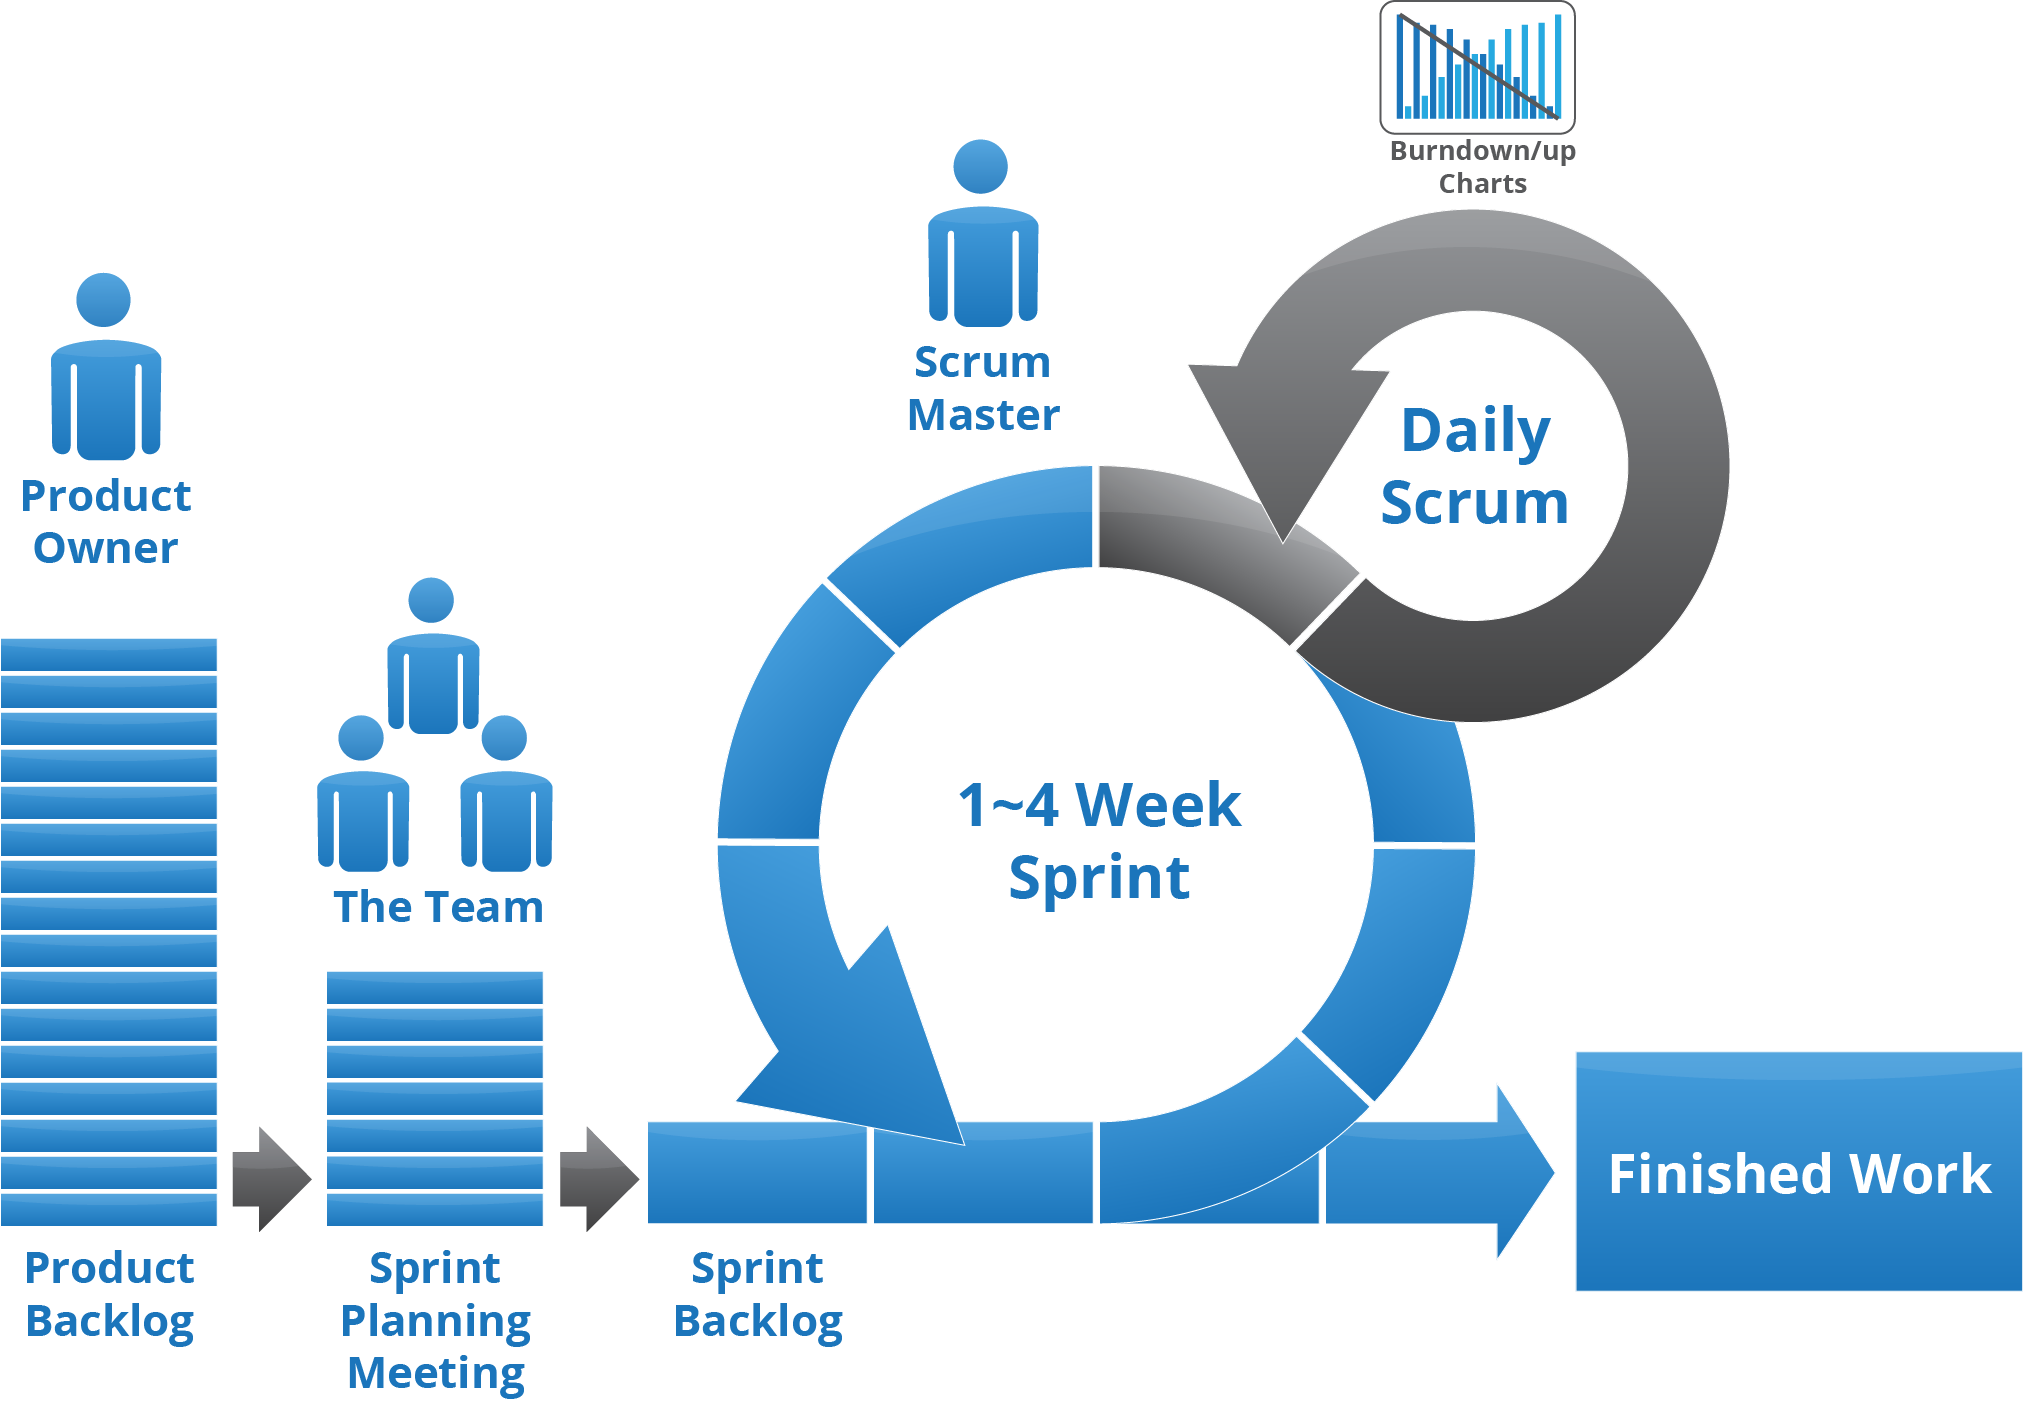
\includegraphics[scale=0.15]{images/scrum.png}
	\caption{The Scrum Process}\label{fig:scrum}
\end{figure}

\subsection{Theoretical Background}\label{scrum-theoretical-background}

\begin{flushleft}
	The original scrum guide is considered incomplete by its creators by design.
	Rather than defining detailed instructions to all teams worldwide, the rules
	of Scrum are intended to guide relationships and interactions between the people
	and their work. Founded on empiricism and lean thinking, Scrum asserts that
	knowledge comes from experience and making decisions based on what's observed.
	In a nutshell, it Scrum employs an iterative approach to optimize predictability
	and risk control. This methodology requires a cross-functional team working
	intensely together. Another positive side effect of this collaboration effort
	is that members of the team are encouraged to acquire and share knowledge together.
\end{flushleft}

\subsection{Transparency}\label{scrum-transparency}

\begin{flushleft}
	The emergent process and work must be visible to those performing the work
	as well as those receiving the work. With Scrum, important decisions are based
	on the perceived state of its three formal artifacts. Artifacts that have low
	transparency can lead to decisions that diminish value and increase risk.
	Transparency enables inspection. Inspection without transparency is misleading
	and wasteful.
\end{flushleft}

\subsection{Inspection}\label{scrum-inspection}

\begin{flushleft}
	The Scrum artifacts and the progress toward agreed goals must be inspected
	frequently and diligently to detect potentially undesirable variances or problems.
	To help with inspection, Scrum provides cadence in the form of its five events.
	Inspection enables adaptation. Inspection without adaptation is considered pointless.
	Scrum events are designed to provoke change.
\end{flushleft}

\subsection{Adaption}\label{scrum-adaption}

\begin{flushleft}
	If any aspects of a process deviate outside acceptable limits or if the resulting
	product is unacceptable, the process being applied or the materials being produced
	must be adjusted. The adjustment must be made as soon as possible to minimize
	further deviation. Adaptation becomes more difficult when the people involved are
	not empowered or self-managing. A Scrum Team is expected to adapt the moment it
	learns anything new through inspection.
\end{flushleft}

\subsection{Scrum Values}\label{scrum-values}

\begin{flushleft}
	Successful use of Scrum depends on people becoming more proficient in living five values:
\end{flushleft}

\begin{enumerate}
	\item Commitment
	\item Focus
	\item Openness
	\item Respect
	\item Courage
\end{enumerate}

\begin{flushleft}
	The primary focus of the Scrum team is on the work of the Sprints to make the
	best possible progress toward these goals. Both the team and the stakeholder
	are open about the work and the challenges involved. These value give direction
	to the Scrum Team with regard to their work, actions and behavior. Decisions
	being made should reinforce and not diminish these values; only when these
	values are embodied, the empirical Scrum pillars of transparency, inspection
	and adaption come to life building trust.
\end{flushleft}

\subsection{Scrum Team}\label{scrum-team}

\begin{flushleft}
	The Scrum team is fundamental to Scrum without it no work would get done.
	This team largely consists of three types of people whose roles are described
	in more detail in the subsections below. Ideally, you'd want to keep this
	team small enough to remain nimble and large enough to be able to complete the
	work within the designated time period. As a rule of thumb, 10 or fewer people
	make up such a team.
\end{flushleft}

\begin{flushleft}
	In the event that a team grows too much in size, consider reorganizing into
	multiple cohesive teams, each focused on the same product and sharing the same
	Product Goal, Product Backlog and Product Owner. The responsibilities that fall
	into the hand of the Scrum team includes:
\end{flushleft}

\begin{itemize}
	\item Product-related activities from stakeholder collaboration
	\item Verification
	\item Experimentation
	\item Research
	\item Development
	\item Anything else that might be required to meet the Product Goal
\end{itemize}

\begin{flushleft}
	Working in Sprints at a sustainable pace helps improve the team's focus and consistency.
\end{flushleft}

\subsection{Product Owner}\label{scrum-product-owner}

\begin{flushleft}
	The Product Owner (a single entity) is accountable for maximizing the value of
	the product resulting from the work of the Scrum Team. How this is done may vary
	widely across organizations, Scrum Teams, and individuals. They are also accountable
	for effective Product Backlog management, which includes:
\end{flushleft}

\begin{itemize}
	\item Developing and explicitly communicating the scrum > Product Goal
	\item Creating and clearly communicating the Product Backlog items
	\item Ordering Product Backlog items
	\item Ensuring that the Product Backlog is transparent, visible and understood
\end{itemize}

\begin{flushleft}
	The Product Owner may do the above work or may delegate the responsibility to
	others. Regardless, the Product Owner remains accountable. The Product Owner
	may represent the needs of many stakeholders in the Product Backlog. Those
	wanting to change the Product Backlog can do so by trying to convince the
	Product Owner because it's the product owner's responsibility to decide whether
	the software goes out at the end of a sprint. In short, the product owner is
	the gatekeeper for everything that comes in and goes out and thus may be
	considered a crucial point in the Scrum process, which is especially true
	from devsecops's points of view. However, it is also the product owner who's
	usually does not receive adequate security training.
\end{flushleft}

\subsection{Developers}\label{scrum-developers}

\begin{flushleft}
	Developers are the people in the Scrum Team that are committed to creating any
	aspect of a usable Increment each Sprint. The specific skills needed by the
	Developers are often broad and will vary with the domain of work. However, the
	Developers are always accountable for:
\end{flushleft}

\begin{itemize}
	\item Creating a plan for the Sprint, namely the Sprint Backlog
	\item Instilling quality by adhering to a Definition of Done
	\item Adapting their plan each day toward a Sprint Goal
	\item Holding each other accountable as professionals
\end{itemize}

\subsection{Scrum Master}\label{scrum-master}

\begin{flushleft}
	The Scrum Master is accountable for establishing Scrum as defined in the Scrum
	Guide. They do this by helping everyone understand Scrum theory and practice,
	both within the Scrum Team and the organization. The Scrum Master serves the
	Scrum Team in several ways, including:
\end{flushleft}

\begin{itemize}
	\item Coaching the team members in self-management and cross-functionality
	\item Helping the Scrum team focus on creating high-value Increments that meet the Definition of Done
	\item Causing the removal of impediments to the Scrum Team's progress
	\item Ensuring that all Scrum events take place and are positive, productive, and kept within the time box
\end{itemize}

\begin{flushleft}
	The Scrum Master serves the Product Owner in several ways, including:
\end{flushleft}

\begin{itemize}
	\item Helping find techniques for effective Product Goal definition and Product Backlog management
	\item Helping the Scrum Team understand the need for clear and concise Product Backlog items
	\item Helping establish empirical product planning for a complex environment
	\item Facilitating stakeholder collaboration as requested or needed
\end{itemize}

\begin{flushleft}
	The Scrum Master serves the organization in several ways, including:
\end{flushleft}

\begin{itemize}
	\item Leading, training, and coaching the organization in its Scrum adoption
	\item Planning and advising Scrum implementations within the organization
	\item Helping employees and stakeholders understand and enact an empirical approach for complex work
	\item Removing barriers between stakeholders and Scrum Teams
\end{itemize}

\subsection{Scrum Events}\label{scrum-events}

\begin{flushleft}
	The Sprint is a container for all other events. Each event in Scrum is a formal
	opportunity to inspect and adapt Scrum Artifacts. These events are specifically
	designed to enable the transparency required. Failure to operate any events as
	prescribed results in lost opportunities to inspect and adapt (see also: Scrum Values).
	Events are used in Scrum to create regularity and to minimize the need for meetings
	not defined in Scrum. Optimally, all events are held at the same time and place
	to reduce complexity.
\end{flushleft}

\subsection{Sprints}\label{scrum-sprints}

\begin{flushleft}
	Sprints are fixed length events of one month or less (typically two weeks in
	length) to create consistency. A new Sprint starts immediately after the conclusion
	of the previous Sprint. All the work necessary to achieve the Product Goal, including
	Sprint Planning, Daily Scrum, Sprint Review, and Sprint Retrospective, happen within
	Sprints. During the sprint no changes are made that would endanger the Sprint Goal,
	nor does the quality of the work decrease. Keep the backlog as refined as needed,
	and clarify and renegotiate the scope with the Product Owner as more is learned.
	Short sprints can be employed to generate more learning cycles and limit risk
	of cost and effort to a smaller time frame. At best, each sprint may be considered
	a small project itself. A sprint could be canceled if the Sprint Goal become
	obsolete, although only the Product Owner has the authority to cancel a sprint.
\end{flushleft}

\subsection{Sprint Planning}\label{scrum=srpint-planning}

\begin{flushleft}
	Sprint Planning initiates the Sprint by laying out the work to be performed
	for the Sprint. This resulting plan is created by the collaborative work of
	the entire Scrum Team. The Scrum Team may also invite other people to attend
	Sprint Planning to provide advice. Sprint Planning is timeboxed to a maximum
	of eight hours for a one-month Sprint. For shorter Sprints, the event is
	usually shorter. Sprint Planning addresses the following topics:
\end{flushleft}

\begin{flushleft}
	\textbf{Why is this Sprint valuable?} The Product Owner proposes how the product
	could increase its value and utility in the current Sprint. The whole Scrum Team
	then collaborates to define a Sprint Goal that communicates why the Sprint is
	valuable to stakeholders. The Sprint Goal must be finalized prior to the end of
	Sprint Planning.
\end{flushleft}

\begin{flushleft}
	\textbf{What can be Done this Sprint?} Through discussion with the Product Owner,
	the Developers select items from the Product Backlog to include in the current
	Sprint. The Scrum Team may refine these items during this process, which increases
	understanding and confidence. Selecting how much can be completed within a Sprint
	may be challenging. However, the more the Developers know about their past performance,
	their upcoming capacity, and their Definition of Done, the more confident they will
	be in their Sprint forecasts.
\end{flushleft}

\begin{flushleft}
	\textbf{How will the chosen work get done?} For each selected Product Backlog item,
	the Developers plan the work necessary to create an Increment that meets the Definition
	of Done. This is often done by decomposing Product Backlog items into smaller work
	items of one day or less. How this is done is at the sole discretion of the Developers.
	No one else tells them how to turn Product Backlog items into Increments of value.
	The Sprint Goal, the Product Backlog items selected for the Sprint, plus the plan
	for delivering them are together referred to as the Sprint Backlog.
\end{flushleft}

\subsection{Daily Scrum}\label{scrum-daily}

\begin{flushleft}
	The purpose of the Daily Scrum is to inspect progress toward the Sprint Goal and
	adapt the Sprint Backlog as necessary, adjusting the upcoming planned work. The
	Daily Scrum is a 15-minute event for the Developers of the Scrum Team. To reduce
	complexity, it is held at the same time and place every working day of the Sprint.
	If the Product Owner or scrum > Scrum Master are actively working on items in the
	Sprint Backlog, they participate as Developers. Daily Scrums improve communications,
	identify impediments, promote quick decision-making, and consequently eliminate the
	need for other meetings. The Daily Scrum is not the only time Developers are allowed
	to adjust their plan. They often meet throughout the day for more detailed discussions
	about adapting or re-planning the rest of the Sprint's work.
\end{flushleft}

\subsection{Sprint Review}\label{scrum-sprint-review}

\begin{flushleft}
	The purpose of the Sprint Review is to inspect the outcome of the Sprint and determine
	future adaptations. The Scrum Team presents the results of their work to key stakeholders
	and progress toward the Product Goal is discussed. During the event, the Scrum Team and
	stakeholders review what was accomplished in the Sprint and what has changed in their
	environment. Based on this information, attendees collaborate on what to do next. The
	Product Backlog may also be adjusted to meet new opportunities. The Sprint Review is
	a working session and the Scrum Team should avoid limiting it to a presentation. The
	Sprint Review is the second to last event of the Sprint and is timeboxed to a maximum
	of four hours for a one-month Sprint. For shorter Sprints, the event is usually shorter.
\end{flushleft}

\subsection{Sprint Retrospective}\label{scrum-sprint-retrospective}

\begin{flushleft}
	The purpose of the Sprint Retrospective is to plan ways to increase quality and
	effectiveness. The Scrum Team inspects how the last scrum > Sprints went with
	regards to individuals, interactions, processes, tools, and their Definition
	of Done. Inspected elements often vary with the domain of work. Assumptions
	that led them astray are identified and their origins explored. The Scrum Team
	discusses what went well during the Sprint, what problems it encountered, and
	how those problems were (or were not) solved. The Scrum Team identifies the most
	helpful changes to improve its effectiveness. The most impactful improvements are
	addressed as soon as possible. They may even be added to the Sprint Backlog for
	the next Sprint. The Sprint Retrospective concludes the Sprint. It is timeboxed
	to a maximum of three hours for a one-month Sprint. For shorter Sprints, the event
	is usually shorter.
\end{flushleft}

\subsection{Artifacts}\label{scrum-artifacts}

\begin{flushleft}
	Scrum's artifacts represent work or value. They are designed to maximize Transparency
	of key information. Thus, everyone inspecting them has the same basis for Adaption.
	Each artifact contains a commitment to ensure it provides information that enhances
	transparency and focus against which progress can be measured:
\end{flushleft}

\begin{itemize}
	\item For the Product Owner it is the Product Goal
	\item For the Sprint Backlog is is the Sprint Goal
	\item For the Increment it is the Definition of Done
\end{itemize}

\begin{flushleft}
	These commitments exist to reinforce empiricism and the Scrum values for the Scrum
	team and their stakeholders.
\end{flushleft}

\subsection{Product Backlog}\label{scrum-product-backlog}

\begin{flushleft}
	The Product Backlog is an emergent, ordered list of what is needed to improve
	the product. It is the single source of work undertaken by the Scrum Team. Product
	Backlog items that can be Done by the Scrum Team within one Sprint are deemed
	ready for selection in a Sprint Planning event. They usually acquire this degree
	of Transparency after refining activities. Product Backlog refinement is the act
	of breaking down and further defining Product Backlog items into smaller more
	precise items. This is an ongoing activity to add details, such as a description,
	order, and size. Attributes often vary with the domain of work. The Developers who
	will be doing the work are responsible for the sizing. The Product Owner may influence
	the Developers by helping them understand and select trade-offs.
\end{flushleft}

\subsection{Product Goal}\label{scrum-product-goal}

\begin{flushleft}
	The Product Goal describes a future state of the product which can serve as a target
	for the Scrum Team to plan against. The Product Goal is in the Product Backlog.
	The rest of the Product Backlog emerges to define ``what'' will fulfill the Product Goal.
\end{flushleft}

\begin{displaycquote}
	A product is a vehicle to deliver value. It has a clear boundary, known stakeholders,
	well-defined users or customers. A product could be a service, a physical product,
	or something more abstract.
\end{displaycquote}

\begin{flushleft}
	The Product Goal is the long-term objective for the Scrum Team. They must fulfill
	(or abandon) one objective before taking on the next.
\end{flushleft}

\subsection{Sprint Backlog}\label{scrum-sprint-backlog}

\begin{flushleft}
	The Sprint Backlog is composed of the Sprint Goal (why), the set of Product Backlog
	items selected for the Sprint (what), as well as an actionable plan for delivering
	the Increment (how). The Sprint Backlog is a plan by and for the Developers. It is
	a highly visible, real-time picture of the work that the Developers plan to accomplish
	during the Sprints in order to achieve the Sprint Goal. Consequently, the Sprint Backlog
	is updated throughout the Sprint as more is learned. It should have enough detail that
	they can inspect their progress in the Daily Scrum.
\end{flushleft}

\subsection{Increment}\label{scrum-increment}

\begin{flushleft}
	An Increment is a concrete stepping stone toward the Product Goal. Each Increment is
	additive to all prior Increments and thoroughly verified, ensuring that all Increments
	work together. In order to provide value, the Increment must be usable. Multiple
	Increments may be created within a Sprint. The sum of the Increments is presented at
	the Sprint Review thus supporting empiricism. However, an Increment may be delivered
	to stakeholders prior to the end of the Sprint. The Sprint Review should never be
	considered a gate to releasing value. Work cannot be considered part of an Increment
	unless it meets the Definition of Done.
\end{flushleft}

\subsection{Definition of Done}\label{scrum-definition-of-done}

\begin{flushleft}
	The Definition of Done is a formal description of the state of the Increment when
	it meets the quality measures required for the product. The moment a Product Backlog
	item meets the Definition of Done, an Increment is born. The Definition of Done
	creates Transparency by providing everyone a shared understanding of what work
	was completed as part of the Increment. If a Product Backlog item does not meet
	the Definition of Done, it cannot be released or even presented at the Sprint Review.
	Instead, it returns to the Product Backlog for future consideration. If the Definition
	of Done for an Increment is part of the standards of the organization, all Scrum Teams
	must follow it as a minimum. If it is not an organizational standard, the Scrum Team
	must create a Definition of Done appropriate for the product. The Developers are
	required to conform to the Definition of Done. If there are multiple Scrum Teams
	working together on a product, they must mutually define and comply with the same
	Definition of Done.
\end{flushleft}


% === End Section Includes ====

\end{document}
